\chapter{Project management}

\label{ch:management}
\lhead{Chapter 2. \emph{Project management}}

This chapter describes the planning of the project. Section \ref{section:planning} is about project planning,
section \ref{section:organization} covers project organizazion.

\section{Project planning}
\label{section:planning}
This section describes the planning of the project including schedule, resources and tool selection.

\subsection{Project goals}
The project has various goals. One is the delivery of a report that describes the all phases and relevant aspects regarding the development of the project. Another one is the development of the integration platform together with two or three prototype applications which can be used to demonstrate the functionality of the system and possibily stimulate further development of a national integration platform for eHealth.

Expected deliverables:

\begin{itemize}
\item Project report
\item Integration platform
\item Two or three prototype applications
\end{itemize}


%\subsection{Limitations}

\subsection{Project schedule}

\textbf{Milestones} \newline
We have identified four milestones for the project. These are associated with important events in the project lifetime and can help us to better monitor its progress. Project's milestones are shown in table \ref{table:milestones}.

\begin{table}[h]
\begin{center}
\begin{tabular}{ | l | l | l | }
  \hline
  Milestone & Date & Description \\
  \hline\noalign{\smallskip}\noalign{\smallskip}\hline
  M1 & 20.09.2013 & Basic implementation of the platform and one prototype. \\ 
  M2 & 08.10.2013 & Mid-term report delivery. \\
  M3 & 04.11.2013 & Feature freeze. \\
  M4 & 21.11.2013 & Project demonstration. Final report delivery. \\
  \hline
\end{tabular}
\end{center}
\caption{Project milestones}
\label{table:milestones}
\end{table}

\textbf{Sprints schedule} \newline
Table \ref{table:sprints} contains an overview of the Sprints in the project.

\begin{table}[h]
\begin{center}
\begin{tabular}{ | l | l | l | }
  \hline
  Sprint & Start date & End date \\
  \hline\noalign{\smallskip}\noalign{\smallskip}\hline
  0 &  &  \\ 
  1 & 09.09.2013 & 22.09.2013 \\
  2 & 23.09.2013 & 06.10.2013 \\
  3 & 07.09.2013 & 20.10.2013 \\
  4 & 21.10.2013 & 04.11.2013 \\
  5 & 05.11.2013 & 21.11.2013 \\
  \hline
\end{tabular}
\end{center}
\caption{Planned sprints}
\label{table:sprints}
\end{table}

\subsection{Work plan}
\newpage
\begin{landscape}
\begin{figure}[h]
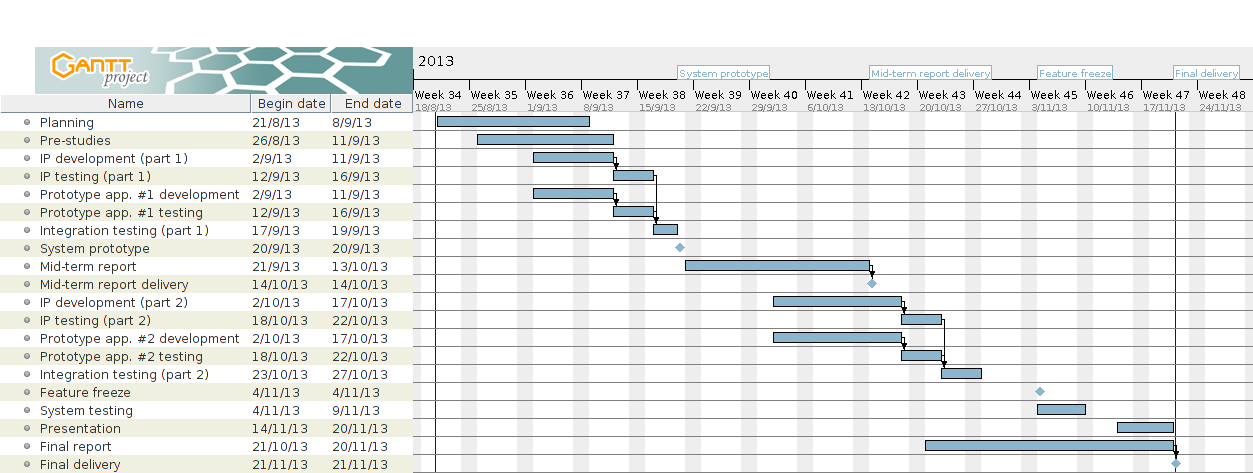
\includegraphics[scale=0.66]{../Figures/gantt-diagram.png}
\caption{Gantt diagram}
\label{figure:work-splan}
\end{figure}
\end{landscape}

\subsection{Resources}
The team consists of three members from different educational backgrounds and with different skills.
We have thus created a skill matrix regarding the technologies involved in the project in order to better distribute the work among us.
The skills are valued on a scale of zero to five based on criterias according to table \ref{table:skillscale}.
Each value corresponds to a certain degree of proficiency, detailed in table \ref{table:proficiency}.
The skill matrix is shown in table \ref{table:skillmatrix}.

\begin{table}[h]
\begin{center}
\begin{tabular}{ | c | l | l | }
  \hline
  Level & Proficiency & Criteria \\
  \hline\noalign{\smallskip}\noalign{\smallskip}\hline
  0 & None		& Has no clue what we're talking about. \\
  1 & Basic		& Has read about it.\\
  2 & Fair		& Has studied it at school.\\
  3 & Good		& Personal interest, use in small-medium sized projects.\\
  4 & Very good	& Strong personal interest, use in medium-large sized projects. \\
  5 & Excellent	& 10+ Years of work experience. \\
  \hline
\end{tabular}
\end{center}
\caption{Skill's scale explanation}
\label{table:skillscale}
\end{table}

\begin{table}[h]
\begin{center}
\begin{tabular}{ | l | l | }
  \hline
  Proficiency & Description \\
  \hline\noalign{\smallskip}\noalign{\smallskip}\hline
  None		& Cannot perform the task \\
  Basic		& Can perform the task with some help from other people \\
  Fair		& Can perform the task almost indipendently \\
  Good		& Can perform the task without any help \\
  Very good	& Can help others to complete the task \\
  Excellent	& Can help others to complete the task \\
  \hline
\end{tabular}
\end{center}
\caption{Proficiency level description}
\label{table:proficiency}
\end{table}

\begin{table}[h]
\begin{center}
\begin{tabular}{ | l | c | c | c | c | c | c | c | c | }
  \hline
  Team member & Java & JS & Android & Database & CSS & AJAX & Spring & LaTeX \\
  \hline\noalign{\smallskip}\noalign{\smallskip}\hline
  Anders & 4 & 4 & 3 & 4 & 4 & 2 & 3 & 1 \\
  Emanuele & 4 & 1 & 3 & 2 & 1 & 1 & 0 & 3 \\
  Sebastian & ? & ? & ? & ? & ? & ? & ? & ? \\
  \hline
\end{tabular}
\end{center}
\caption{Skill matrix}
\label{table:skillmatrix}
\end{table}

\subsection{Tool selection}
This section will describe the different tools we used throught the project.


\begin{description}

\item[Git and GitHub]
Git is one of the most used version control systems. Although it is mostly used for code, it can be used to manage other types of file such as LaTeX. GitHub is a repository hosting service for Git projects which offers a web-based fronted. We have decided to use Git because of the familiarity we had with it. We used Git for managing both the code and the report.

\item[Sublime Text]
Sublime Text is a popular, cross-platform editor which offers advanced features.
We used Sublime Text for editing the report and for coding JavaScript, CSS and AJAX.

\item[IntelliJ IDEA]
A popular, feature-rich Java IDE. We used it to develop the Android applications and for Spring coding.

\item[Apache Maven]
Maven is an open and cross-platform build system for Java projects which, among other things, takes care of dependecies. Maven is powerful and well documented and seemed an optimal choice for our project also because of the familiarity we had with it.

\item[LaTeX suite]
LaTeX is a powerful language used to prepare documents which is widely used in academical environments. LaTeX takes care of the formatting of the document allowing the writer to focus on the contents, moreover LaTeX documents can be written with any text editor.
We chose LaTeX because of the familiarity we had with it.
%LaTeX files can then be compiled to PDF files.

\item[Google Drive and Google Docs]
Google Drive is a service which lets you access your files from everywhere and share them with other people. It is tightly integrated with Google Docs, a web-based productivity suite. We used Google Drive to share documents within the team and with the customer and supervisor.
Many of the documents and diagrams produced for the project were created using Google Docs.

\item[Skype]
A popular instant-messaging client that also supports audio and video communication.
Skype was used throught the project to keep in touch with the customer and team members.

\item[Travis CI]
Travis CI is an automated build service...
% we should write two more lines here.

\item[Facebook]
Facebook is a social networking service. The team created a group on Facebook that was used as a bulleting board for internal communications.

%\item[Violet UML] A free UML editor.
%Balsamiq Mockups looks great, it would be cool to do some mockup with this!!
%Lucidchart maybe we can opt for a free solution like violet UML.

\end{description}


\section{Project organization}
\label{section:organization}
This section describes the organizational aspects of the project such as roles description, allocation and meetings schedule.

\subsection{Role description}
We have identified a number of roles in this project. Although each role has different, distinct responsabilities, we see all roles as equally important for the success of this project.

\begin{description}
\item[Project manager]
\item[Scrum master]
\item[Product owner]
%\item[Document responsible]
%\item[System architect]
%\item[]
\item[Secretary]
Responsible for taking notes during meetins and booking rooms.
\item[Quality assurance]
Ensures that quality practices are in place and use.
\item[Web developer]
Responsible for web development.
\item[Droid developer]
Responsible for Android development.
\item[Supervisor relations]
Responsible for communication with the supervisor.
\item[Customer relations]
Responsible for contacting the customer.
\end{description}

\subsection{Role allocation}
Roles were allocated mostly basing on team members' competences.
Those roles that were left unassigned were taken up by members who volunteered for them upon approval of other team members.
Because we were only three people, all of us had more than one role. Sometimes, roles were shared.

\begin{table}
\begin{center}
\begin{tabular}{ | l | l | }
  \hline
  Member & Roles \\
  \hline\noalign{\smallskip}\noalign{\smallskip}\hline
  Anders Olsen Sandvik  &  \\
  Emanuele Di Santo     &  \\
  Sebastian Zalewski    &  \\
  \hline
\end{tabular}
\end{center}
\caption{Members' roles}
\label{table:roles}
\end{table}

\subsection{Weekly schedule}
During the early stages of the project the team has agreed on a meeting schedule.

\begin{description}
\item[Monday] \hfill from 10 to 19 \\
\textbf{Weekly startup meeting} from 1000 to 1100.\newline
At the begin of each week we would review the progress done during the previous and discuss the plan for the next.
We also discussed any problems encountered.
This internal meeting would follow the last Status Report document.
\textbf{Customer meeting} from 1100 to 1200.\newline
During the meeting with customer we would discuss with him the work done and share our plan for the next week.
This was done in order to help us prioritize our work to better suit the customer's interest.
\textbf{Supervisor meeting} from 1200 to 1300.
\item[Wednesday] \hfill \\
\textbf{Collective work session} from 15 to 1900. (4 hours)
\end{description}


\section{Quality assurance}
\subsection{Templates}
\subsection{Customer relations}
\subsection{Supervisor relations}

\section{Risk management}

The risk analysis is good but we can improve it with some strategy to handle the risk once it has happened.
